\section{Newsfeed App - Recherchebericht}
\label{section:realisation:newsfeed_app}


Newsfeed App for deskless/frontline employees Firstline workers
\begin{itemize}
\item {Mircosoft Staffhub https://products.office.com/de-de/microsoft-staffhub/staff-scheduling-software}
\item {Inkling 	https://www.inkling.com/ }
\item {Zinc https://www.zinc.it/ Beliebteste/Am häufigsten genutzte App für „Deskless“ Mitarbeiter}
\item {Slack https://slack.com/intl/de-de Desktop worker or/and Frontline worker?}
\item {Nicht geeignet: Whatsapp Business https://www.deutsche-handwerks-zeitung.de/whatsapp-betrieblich-nutzen-was-beim-datenschutz-wirklich-gilt/150/3101/363865}
\end{itemize}

\begin{figure}[H] 
\centering 
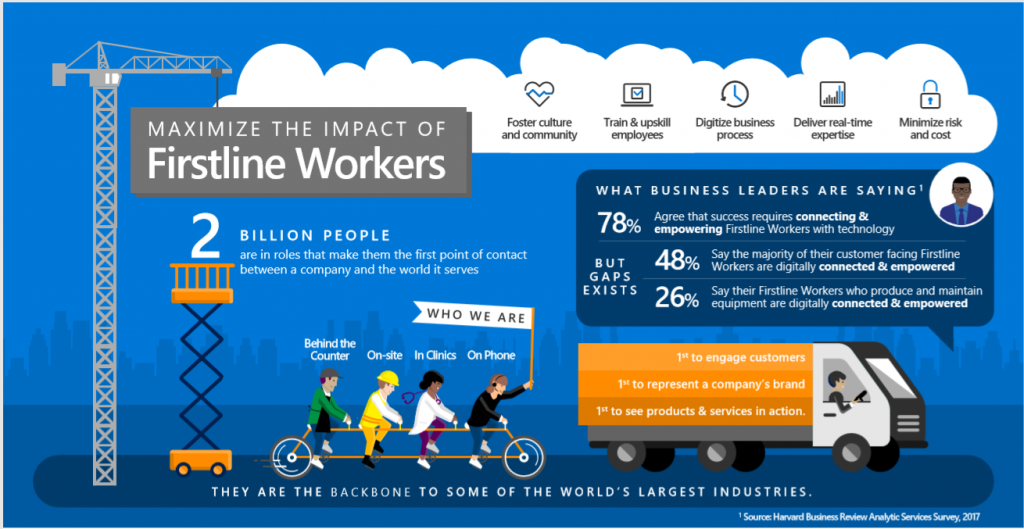
\includegraphics[scale=0.48]{images/frontlineworkers} 
\caption[Frontline Workers]{Frontline workers\protect} 
\label{dem} 
\end{figure}

\subsection{Lastenheft}
\begin{itemize}
\item Es ist ein Recherchebericht zu erstellen, der sich mit Produkten, Lösungen und Anwendungen (im Folgenden als Anwendungen zusammengefasst) befasst. Konkret geht es um Anwendungen, die es Unternehmen ermöglichen, ihre Mitarbeiter über unternehmensinterne Vorgänge zu informieren und den Mitarbeitern eine Interaktion mit dem Unternehmen ermöglichen. 
\item Der Bericht soll eine Übersicht über die am Markt etablierten Anwendungen liefern. Ein Fokus soll auf den Anreizen liegen, mit welchen die Anwendungen die Mitarbeiter zur Benutzung motivieren.
\item Des Weiteren soll im Bericht untersucht werden, welche Umfragefunktionalitäten in der jeweiligen Anwendung bereits existieren und wie diese potentiell durch PulseShift genutzt werden könnten. 
\item Darüber hinaus soll der Bericht aufzeigen, welche weiteren Möglichkeiten zur Einbindung einer Umfrage durch PulseShift es jeweils gibt und wie flexibel diese Möglichkeiten genutzt werden können.
\item Außerdem sollen in dem Bericht die Erfahrungen von Referenzkunden, die die Anwendung bei Offline-Mitarbeitern einsetzen, beschrieben werden. 
\item Sofern jeweils eine Preisstruktur verfügbar ist, soll außerdem auf diese eingegangen werden.
\end{itemize}

\subsection{Pflichtenheft}
\begin{itemize}
\item Es wird ein Recherchebericht erstellt, der sich mit Produkten, Lösungen und Anwendungen (im Folgenden als Anwendungen zusammengefasst) befasst. Konkret wird es um Anwendungen gehen, die es Unternehmen ermöglichen, ihre Mitarbeiter über unternehmensinterne Vorgänge zu informieren und den Mitarbeitern eine Interaktion mit dem Unternehmen ermöglichen.
\item Der Bericht wird eine Übersicht über die am Markt etablierten Anwendungen liefern. Für die Marktführer wird herausgearbeitet, mit welchen Anreizen sie die Mitarbeiter zur Benutzung der Anwendung motivieren. Sofern jeweils möglich werden die Anwendungen dazu neben einer Internetrecherche auch aktiv getestet.
\item Des Weiteren werden im Bericht die Möglichkeiten zur Integration der Umfrage von PulseShift in die jeweilige Anwendung aufgezeigt. Diese wird tabellarisch mit zusätzlichen erläuternden Texten gegenübergestellt. Dabei wird sofern jeweils verfügbar sowohl auf die Umfragefunktionalitäten der Anwendung als auch das Abspringen zur Umfragefunktion von PulseShift eingegangen. Außerdem werden jeweils mögliche weitere anwendungsspezifische Möglichkeiten wie beispielsweise ein Einbinden der Umfrage mittels iFrame vorgestellt.
\item Abschließend werden die Erfahrungen von Referenzkunden dargelegt. Dabei wird der Fokus auf Erfahrungen liegen, die im unmittelbaren Zusammenhang mit dem Einsatz bei Offline-Mitarbeitern stehen.
\item Der Bericht wird innerhalb des Projektabschlussberichts in Latex erstellt.
\end{itemize}
